\documentclass[
	% -- opções da classe memoir --
	12pt,				% tamanho da fonte
	openright,
	oneside,			% para impressão em verso e anverso. Oposto a oneside
	a4paper,			% tamanho do papel. 
	% -- opções da classe abntex2 --
	chapter=TITLE,		% títulos de capítulos convertidos em letras maiúsculas
	%section=TITLE,		% títulos de seções convertidos em letras maiúsculas
	%subsection=TITLE,	% títulos de subseções convertidos em letras maiúsculas
	%subsubsection=TITLE,% títulos de subsubseções convertidos em letras maiúsculas
	% -- opções do pacote babel --
	brazil				% o último idioma é o principal do documento
	]{abntex2}

\setcounter{secnumdepth}{3}
% ---
% Pacotes básicos 
% ---
\usepackage{lmodern}			% Usa a fonte Latin Modern			
\usepackage[T1]{fontenc}		% Selecao de codigos de fonte.
\usepackage[utf8]{inputenc}		% Codificacao do documento (conversão automática dos acentos)
\usepackage{lastpage}			% Usado pela Ficha catalográfica
\usepackage{indentfirst}		% Indenta o primeiro parágrafo de cada seção.
\usepackage{color}				% Controle das cores
\usepackage{graphicx}			% Inclusão de gráficos
\usepackage{microtype} 			% para melhorias de justificação
\usepackage{float}
% ---
		
% ---
% Pacotes adicionais, usados apenas no âmbito do Modelo Canônico do abnteX2
% ---
\usepackage{lipsum}				% para geração de dummy text
% ---

\usepackage{tabularx} % in the preamble

% ---
% Pacotes de citações
% ---
\usepackage[brazilian,hyperpageref]{backref}	 % Paginas com as citações na bibl
\usepackage[alf]{abntex2cite}	% Citações padrão ABNT




% ---
% Informações de dados para CAPA e FOLHA DE ROSTO
% ---
\titulo{Documento de Requisitos:\\ Controle de prestação de serviço - Any@Bike}
\autor{UNIVERSIDADE ESTADUAL DO MATO GROSSO DO SUL\\ CURSO DE CIÊNCIA DA COMPUTAÇÃO}
\local{Dourados}
\data{Novembro de 2015}
\instituicao{Responsável pelo Projeto:\par Felipe Lima Morais}

% O preambulo deve conter o tipo do trabalho, o objetivo, 
% o nome da instituição e a área de concentração 
\preambulo{Trabalho acadêmico apresentado à disciplina de Análise e Projeto de Sistemas, do curso de Bacharelado em Ciência da Computação como requisito parcial para obtenção da nota do quarto bimestre.\newline \newline Profa. Dra. Glaucia Gabriel Sass}
% ---

% alterando o aspecto da cor azul
\definecolor{blue}{RGB}{0,0,0}

% informações do PDF
\makeatletter
\hypersetup{
     	%pagebackref=true,
		pdftitle={\@title}, 
		pdfauthor={\@author},
    	pdfsubject={\imprimirpreambulo},
	    pdfcreator={LaTeX with abnTeX2},
		pdfkeywords={abnt}{latex}{abntex}{abntex2}{trabalho acadêmico}, 
		colorlinks=true,       		% false: boxed links; true: colored links
    	linkcolor=blue,          	% color of internal links
    	citecolor=blue,        		% color of links to bibliography
    	%filecolor=magenta,      		% color of file links
		urlcolor=blue,
		bookmarksdepth=4
}
\makeatother
% --- 

% --- 
% Espaçamentos entre linhas e parágrafos 
% --- 

% O tamanho do parágrafo é dado por:
\setlength{\parindent}{1.3cm}

% Controle do espaçamento entre um parágrafo e outro:
\setlength{\parskip}{0.2cm}  % tente também \onelineskip

% ---
% compila o indice
% ---
\makeindex							%TODO
% ---

% ----
% Início do documento
% ----
\begin{document}

% Seleciona o idioma do documento (conforme pacotes do babel)
%\selectlanguage{english}
\selectlanguage{brazil}

% Retira espaço extra obsoleto entre as frases.
\frenchspacing 

% ----------------------------------------------------------
% ELEMENTOS PRÉ-TEXTUAIS
% ----------------------------------------------------------
% \pretextual

% ---
% Folha de rosto
% (o * indica que haverá a ficha bibliográfica)
% ---
\imprimirfolhaderosto
% ---

% ---
% inserir o sumario
% ---
\pdfbookmark[0]{\contentsname}{toc}
\tableofcontents*
\cleardoublepage
% ---


% ----------------------------------------------------------
% ELEMENTOS TEXTUAIS
% ----------------------------------------------------------
\textual


% ---
% inserir lista de ilustrações
% ---
\pdfbookmark[0]{\listfigurename}{lof}
\addcontentsline{toc}{chapter}{Lista de Figuras}
\listoffigures*
\cleardoublepage
% ---

\chapter{Diagrama de Classe de Projeto}

\begin{figure}[h!]
	\caption{Diagrama de Classes}
	\begin{center}
	    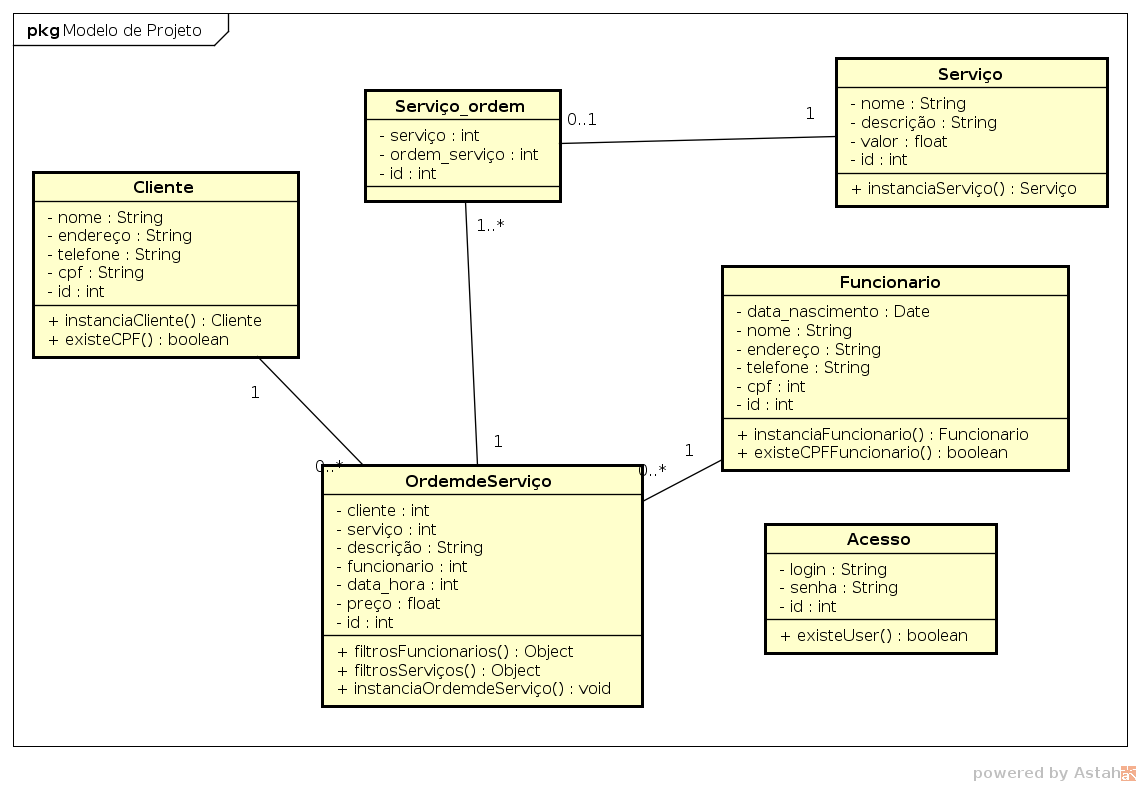
\includegraphics[scale=0.5]{Arquivos/diagrama_classes}  
	\end{center}
	\legend{Fonte:Elaborado pelo autor}
\end{figure}

\section{Diagrama de Transição de Estado}

\begin{figure}[h!]
\subsection{Diagrama de Transição de Estado da classe Cliente}
	\caption{Diagrama de Transição de Estado da classe Cliente}
	\begin{center}
	    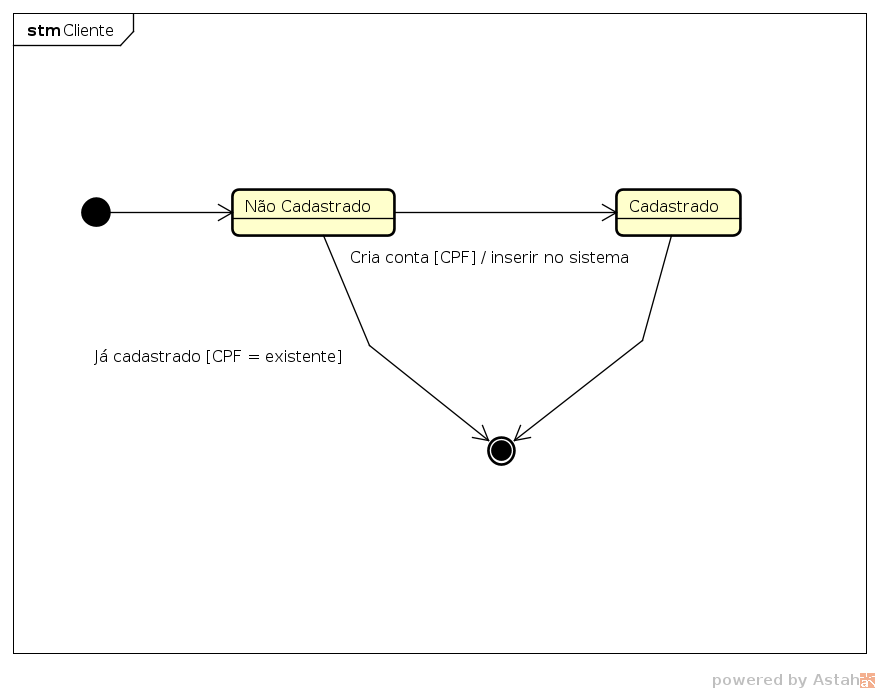
\includegraphics[scale=0.6]{Arquivos/DTE/Cliente}  
	\end{center}
	\legend{Fonte:Elaborado pelo autor}
\end{figure}

\begin{figure}[h!]
\subsection{Diagrama de Transição de Estado da Serviço }
	\caption{Diagrama de Transição de Estado da Serviço}
	\begin{center}
	    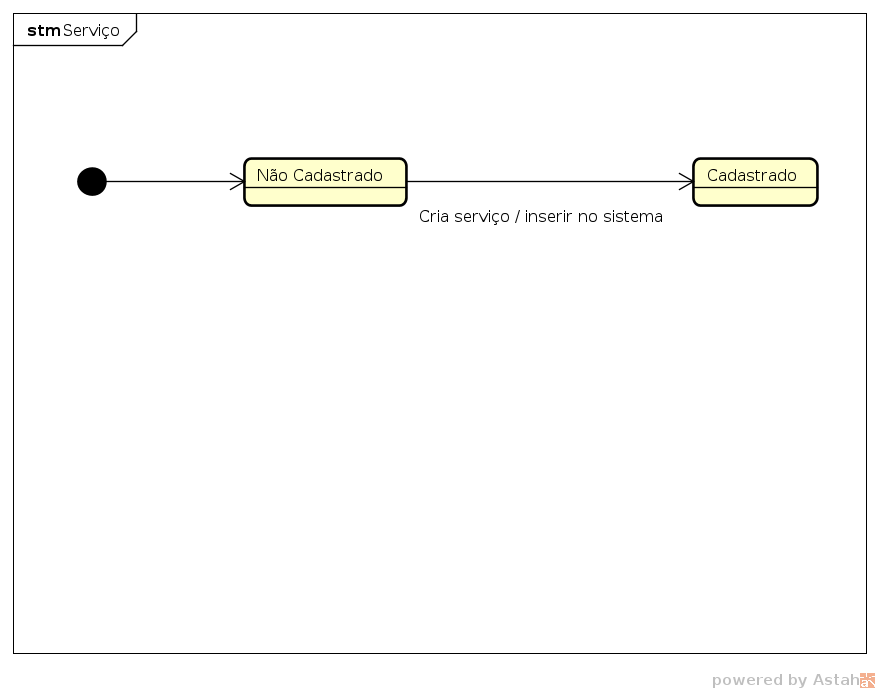
\includegraphics[scale=0.6]{Arquivos/DTE/Servico}  
	\end{center}
	\legend{Fonte:Elaborado pelo autor}
\end{figure}


\begin{figure}[h!]
\subsection{Diagrama de Transição de Estado da classe Funcionario}
	\caption{Diagrama de Transição de Estado da classe Funcionario}
	\begin{center}
	    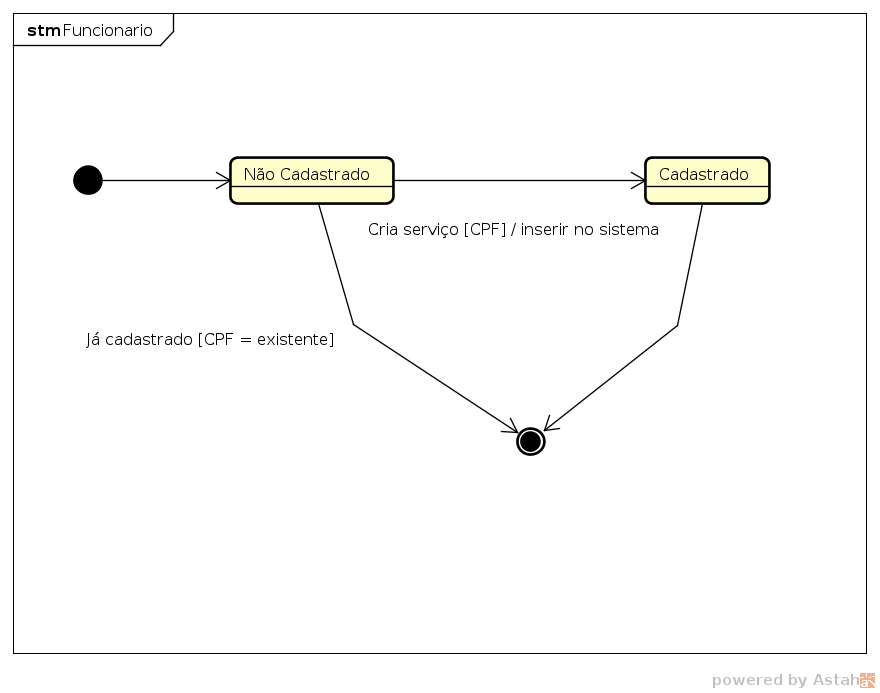
\includegraphics[scale=0.6]{Arquivos/DTE/Funcionario}  
	\end{center}
	\legend{Fonte:Elaborado pelo autor}
\end{figure}

\begin{figure}[h!]
\subsection{Diagrama de Transição de Estado da classe OrdemDeServiço}
	\caption{Diagrama de Transição de Estado da classe OrdemDeServiço}
	\begin{center}
	    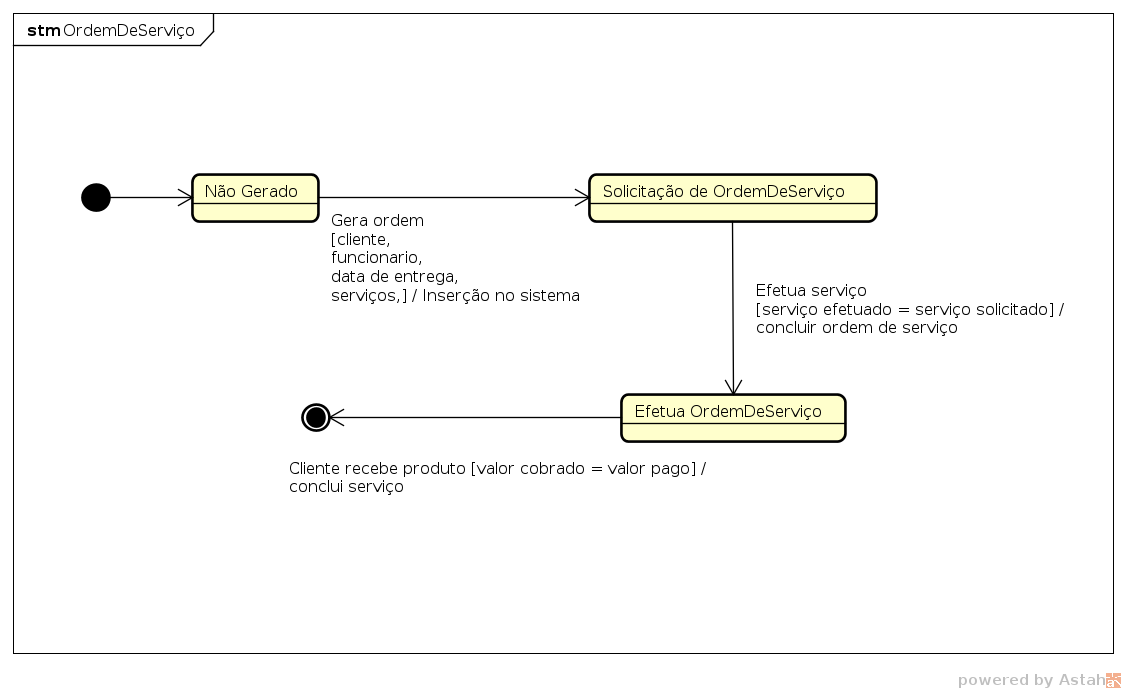
\includegraphics[scale=0.5]{Arquivos/DTE/OrdemDeServico}  
	\end{center}
	\legend{Fonte:Elaborado pelo autor}
\end{figure}

\begin{figure}[h!]
\subsection{Diagrama de Transição de Estado da classe Acesso}
	\caption{Diagrama de Transição de Estado da classe Acesso}
	\begin{center}
	    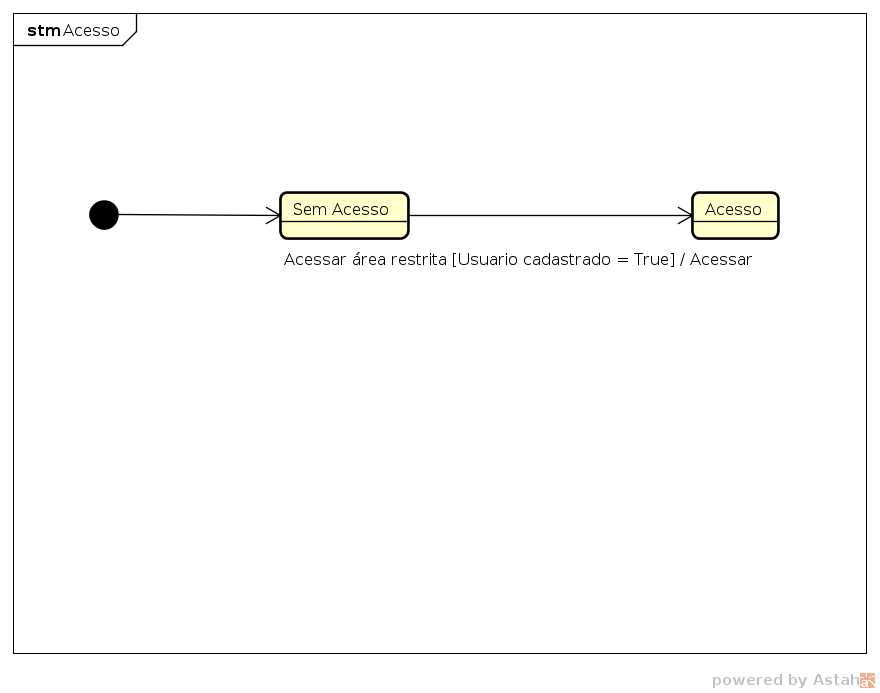
\includegraphics[scale=0.6]{Arquivos/DTE/Acesso}  
	\end{center}
	\legend{Fonte:Elaborado pelo autor}
\end{figure}


\chapter{Diagrama de Casos de Uso}

\begin{figure}[htb]
	\caption{Diagrama modelo de casos de uso}
	\begin{flushleft}
	    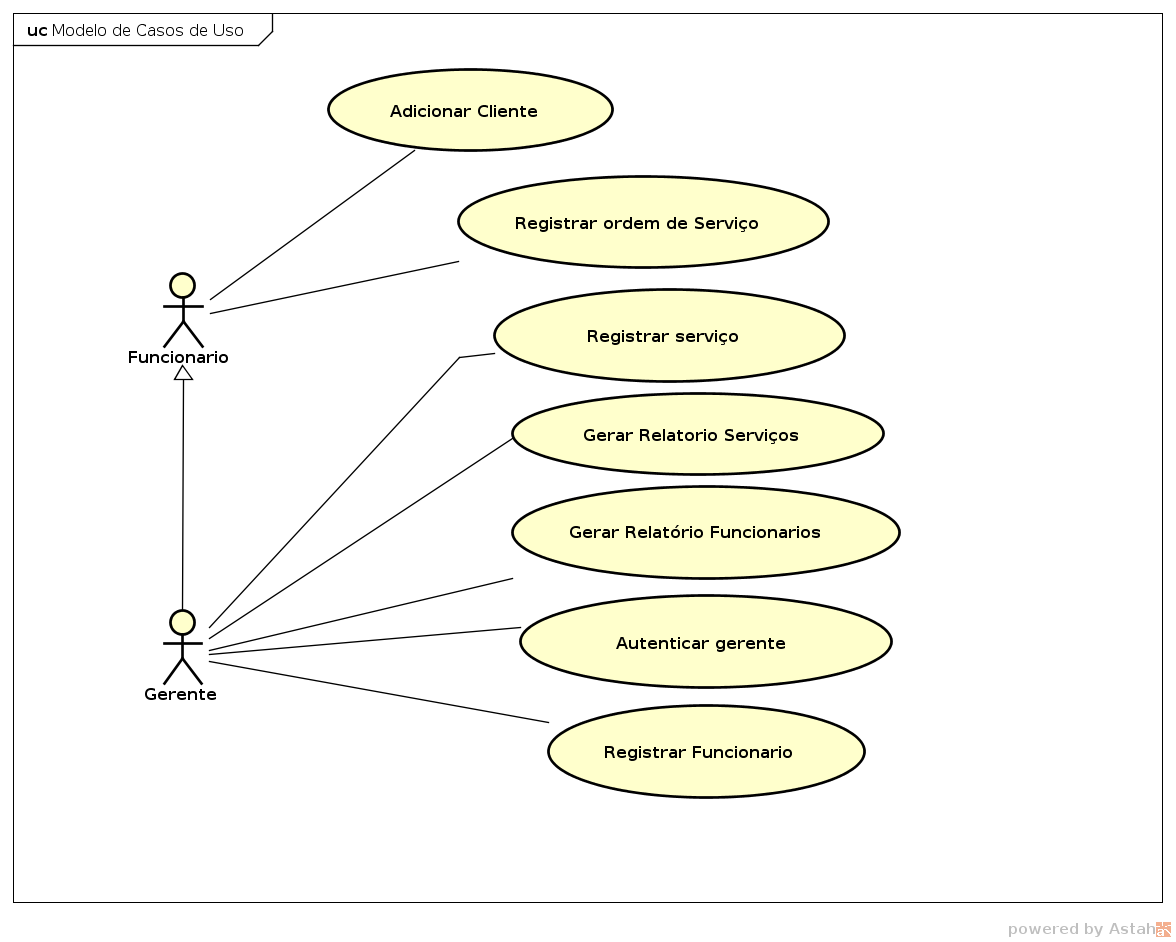
\includegraphics[scale=0.5]{Arquivos/caso_de_uso}  %TODO
	\end{flushleft}
	\label{fig:caso_de_uso}
	\legend{Fonte:Elaborado pelo autor}
\end{figure}

\section{Diagrama de Atividade}

\begin{figure}[h!]
\subsection{Diagrama de Atividade Adicionar Cliente}
	\caption{Diagrama de Atividade Adicionar Cliente}
	\begin{center}
	    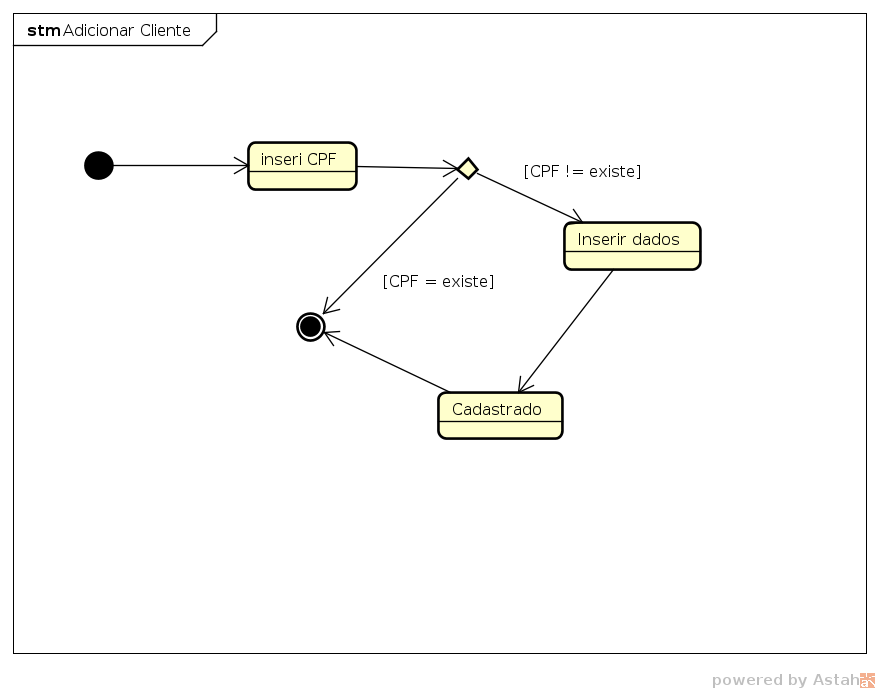
\includegraphics[scale=0.6]{Arquivos/DTE/Adicionar_Cliente}  
	\end{center}
	\legend{Fonte:Elaborado pelo autor}
\end{figure}


\begin{figure}[h!]
\subsection{Diagrama de Atividade Registrar Ordem de Serviço}
	\caption{Diagrama de Atividade Registrar Ordem de Serviço}
	\begin{center}
	    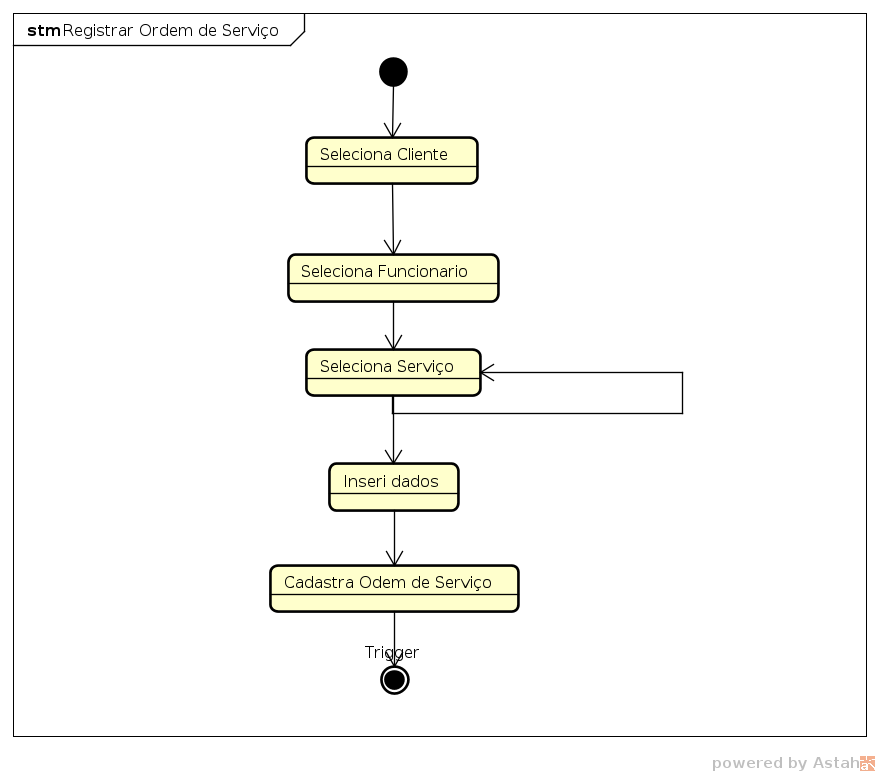
\includegraphics[scale=0.6]{Arquivos/DTE/Registrar_Ordem_de_Servico}  
	\end{center}
	\legend{Fonte:Elaborado pelo autor}
\end{figure}



\begin{figure}[h!]
\subsection{Diagrama de Atividade Registrar Serviço}
	\caption{Diagrama de Atividade Registrar Serviço}
	\begin{center}
	    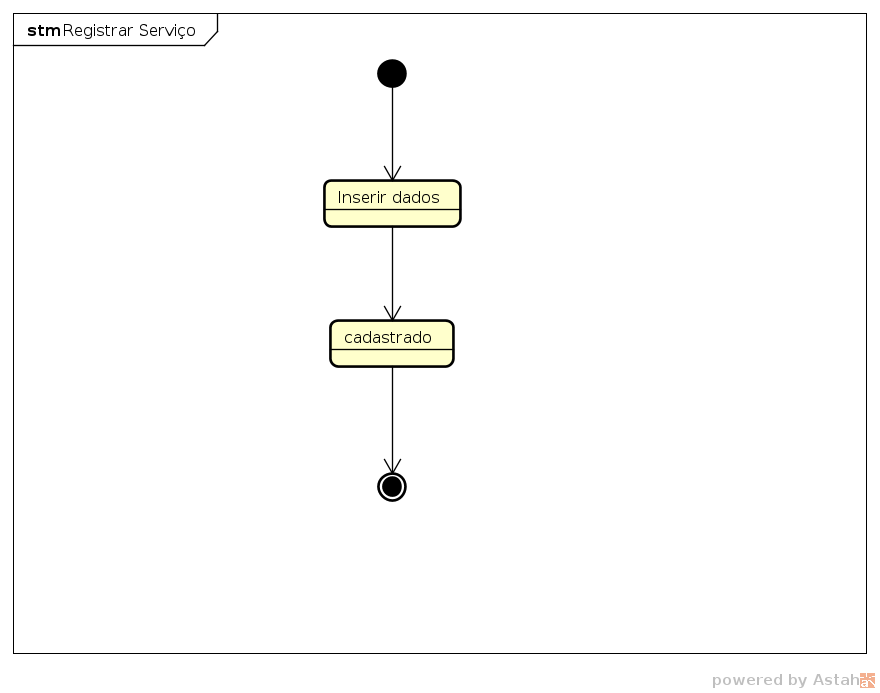
\includegraphics[scale=0.6]{Arquivos/DTE/Registrar_Servico}  
	\end{center}
	\legend{Fonte:Elaborado pelo autor}
\end{figure}



\begin{figure}[h!]
\subsection{Diagrama de Atividade Gerar Relatório de Serviço}
	\caption{Diagrama de Atividade Gerar Relatório de Serviço}
	\begin{center}
	    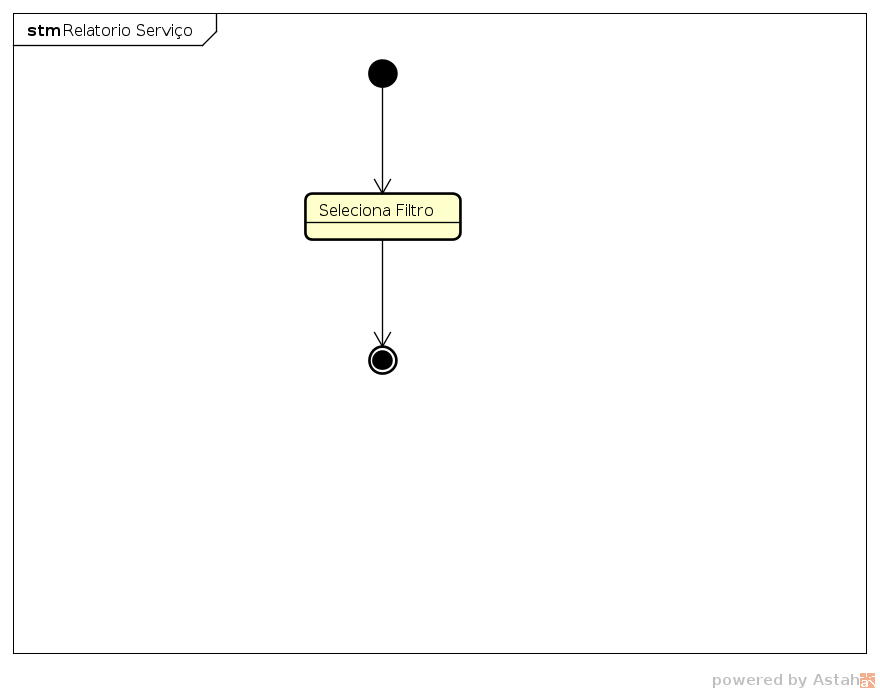
\includegraphics[scale=0.6]{Arquivos/DTE/Relatorio_Servico}  
	\end{center}
	\legend{Fonte:Elaborado pelo autor}
\end{figure}



\begin{figure}[h!]
\subsection{Diagrama de Atividade Gerar Relatório de Funcionarios}
	\caption{Diagrama de Atividade Gerar Relatório de Funcionarios}
	\begin{center}
	    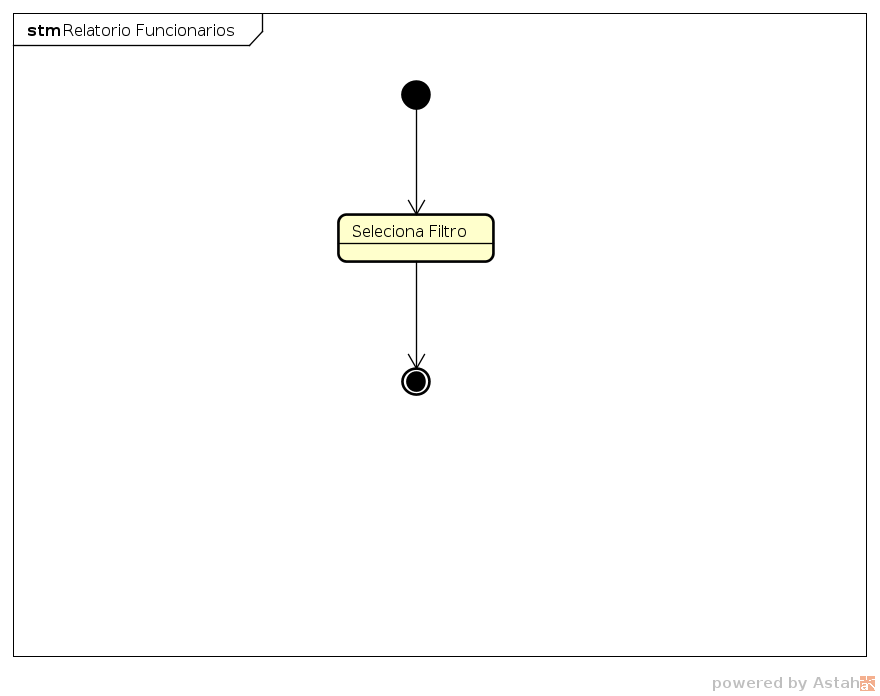
\includegraphics[scale=0.6]{Arquivos/DTE/Relatorio_Funcionarios}  
	\end{center}
	\legend{Fonte:Elaborado pelo autor}
\end{figure}



\begin{figure}[h!]
\subsection{Diagrama de Atividade Autenticar Gerente}
	\caption{Diagrama de Atividade Autenticar Gerente}
	\begin{center}
	    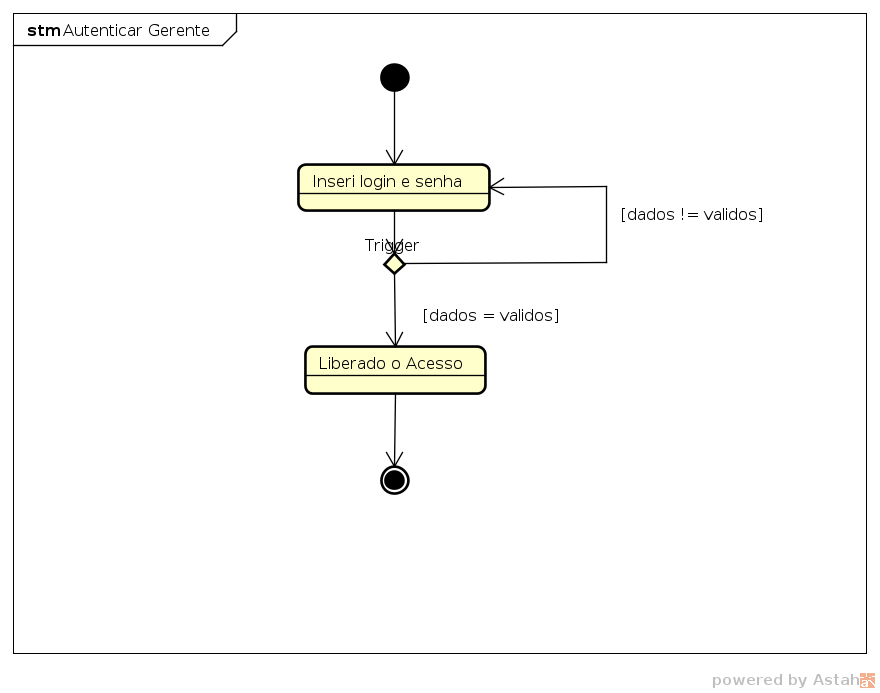
\includegraphics[scale=0.6]{Arquivos/DTE/Autenticar_Gerente}  
	\end{center}
	\legend{Fonte:Elaborado pelo autor}
\end{figure}



\begin{figure}[h!]
\subsection{Diagrama de Atividade Registrar Funcionario}
	\caption{Diagrama de Atividade Registrar Funcionario}
	\begin{center}
	    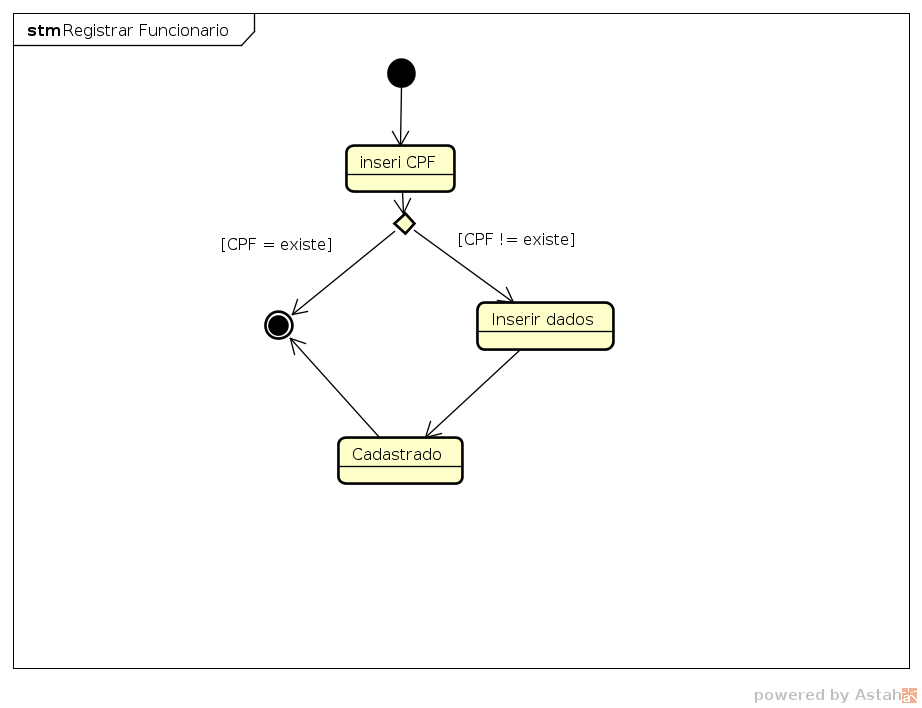
\includegraphics[scale=0.6]{Arquivos/DTE/Registrar_Funcionario}  
	\end{center}
	\legend{Fonte:Elaborado pelo autor}
\end{figure}



\chapter{Mapeamento Objeto Relacional}

\begin{figure}[htb]
	\caption{Mapeamento Objeto Relacional}
	\begin{flushleft}
	    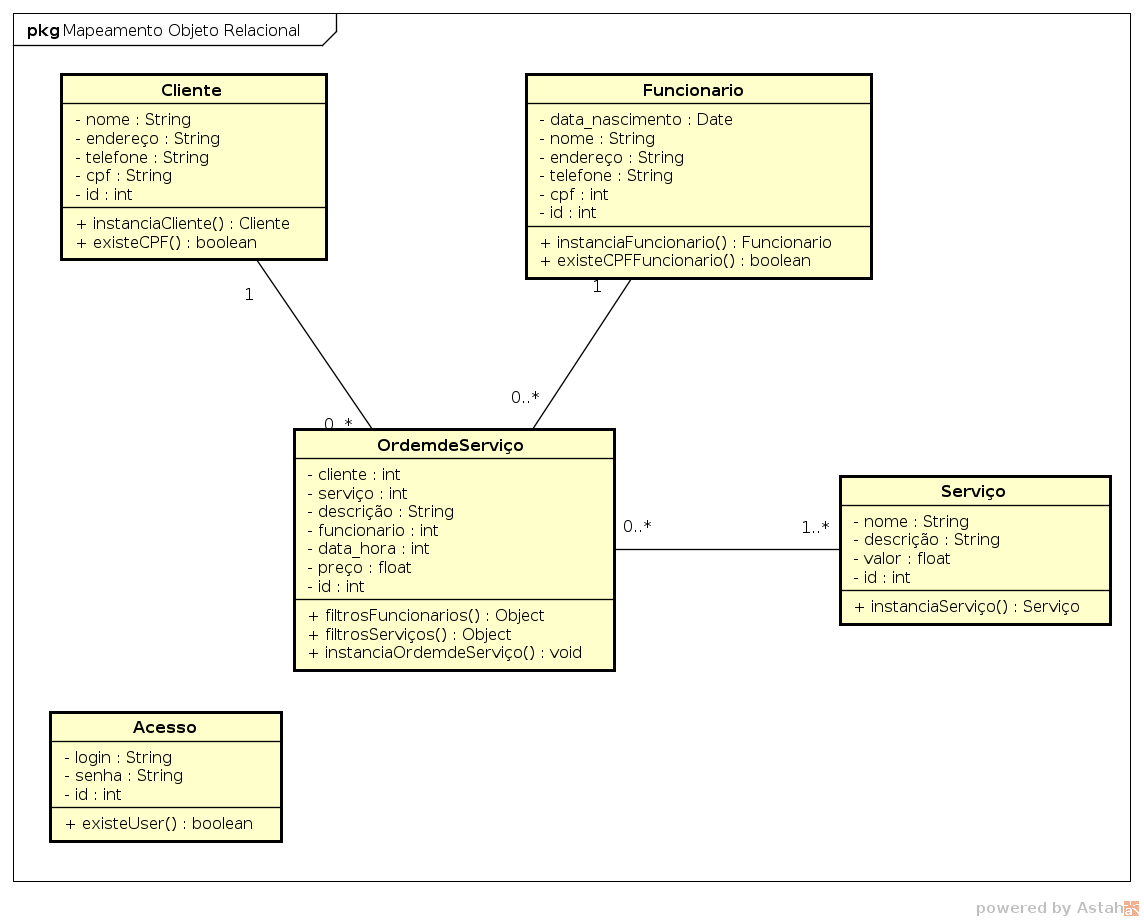
\includegraphics[scale=0.5]{Arquivos/DTE/Mapeamento_Objeto_Relacional}  %TODO
	\end{flushleft}
	\label{fig:caso_de_uso}
	\legend{Fonte:Elaborado pelo autor}
\end{figure}

\end{document}

